% Created by tikzDevice version 0.12.3.1 on 2023-04-12 14:24:53
% !TEX encoding = UTF-8 Unicode
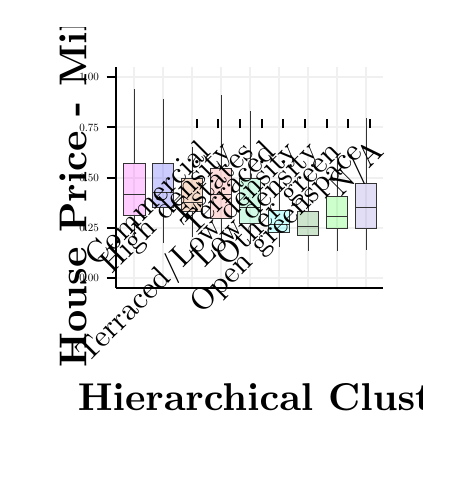
\begin{tikzpicture}[x=1pt,y=1pt]
\definecolor{fillColor}{RGB}{255,255,255}
\path[use as bounding box,fill=fillColor,fill opacity=0.00] (0,0) rectangle (142.64,152.15);
\begin{scope}
\path[clip] (  0.00,  0.00) rectangle (142.64,152.15);
\definecolor{fillColor}{RGB}{255,255,255}

\path[fill=fillColor] (  0.00,  0.00) rectangle (142.64,152.15);
\end{scope}
\begin{scope}
\path[clip] ( 32.06, 58.04) rectangle (128.41,137.92);
\definecolor{fillColor}{RGB}{255,255,255}

\path[fill=fillColor] ( 32.06, 58.04) rectangle (128.41,137.92);
\definecolor{drawColor}{gray}{0.94}

\path[draw=drawColor,line width= 0.7pt,line join=round] ( 32.06, 61.67) --
	(128.41, 61.67);

\path[draw=drawColor,line width= 0.7pt,line join=round] ( 32.06, 79.82) --
	(128.41, 79.82);

\path[draw=drawColor,line width= 0.7pt,line join=round] ( 32.06, 97.98) --
	(128.41, 97.98);

\path[draw=drawColor,line width= 0.7pt,line join=round] ( 32.06,116.13) --
	(128.41,116.13);

\path[draw=drawColor,line width= 0.7pt,line join=round] ( 32.06,134.29) --
	(128.41,134.29);

\path[draw=drawColor,line width= 0.7pt,line join=round] ( 38.34, 58.04) --
	( 38.34,137.92);

\path[draw=drawColor,line width= 0.7pt,line join=round] ( 48.82, 58.04) --
	( 48.82,137.92);

\path[draw=drawColor,line width= 0.7pt,line join=round] ( 59.29, 58.04) --
	( 59.29,137.92);

\path[draw=drawColor,line width= 0.7pt,line join=round] ( 69.76, 58.04) --
	( 69.76,137.92);

\path[draw=drawColor,line width= 0.7pt,line join=round] ( 80.23, 58.04) --
	( 80.23,137.92);

\path[draw=drawColor,line width= 0.7pt,line join=round] ( 90.71, 58.04) --
	( 90.71,137.92);

\path[draw=drawColor,line width= 0.7pt,line join=round] (101.18, 58.04) --
	(101.18,137.92);

\path[draw=drawColor,line width= 0.7pt,line join=round] (111.65, 58.04) --
	(111.65,137.92);

\path[draw=drawColor,line width= 0.7pt,line join=round] (122.13, 58.04) --
	(122.13,137.92);
\definecolor{drawColor}{gray}{0.20}

\path[draw=drawColor,line width= 0.1pt,line join=round] ( 48.82,103.24) -- ( 48.82,126.44);

\path[draw=drawColor,line width= 0.1pt,line join=round] ( 48.82, 87.14) -- ( 48.82, 74.44);
\definecolor{fillColor}{RGB}{0,0,255}

\path[draw=drawColor,line width= 0.1pt,fill=fillColor,fill opacity=0.20] ( 44.89,103.24) --
	( 44.89, 87.14) --
	( 52.74, 87.14) --
	( 52.74,103.24) --
	( 44.89,103.24) --
	cycle;

\path[draw=drawColor,line width= 0.1pt] ( 44.89, 92.86) -- ( 52.74, 92.86);

\path[draw=drawColor,line width= 0.1pt,line join=round] ( 38.34,103.32) -- ( 38.34,129.97);

\path[draw=drawColor,line width= 0.1pt,line join=round] ( 38.34, 84.55) -- ( 38.34, 76.26);
\definecolor{fillColor}{RGB}{255,0,255}

\path[draw=drawColor,line width= 0.1pt,fill=fillColor,fill opacity=0.20] ( 34.41,103.32) --
	( 34.41, 84.55) --
	( 42.27, 84.55) --
	( 42.27,103.32) --
	( 34.41,103.32) --
	cycle;

\path[draw=drawColor,line width= 0.1pt] ( 34.41, 91.86) -- ( 42.27, 91.86);

\path[draw=drawColor,line width= 0.1pt,line join=round] ( 90.71, 86.06) -- ( 90.71, 97.67);

\path[draw=drawColor,line width= 0.1pt,line join=round] ( 90.71, 78.30) -- ( 90.71, 73.01);
\definecolor{fillColor}{RGB}{0,255,255}

\path[draw=drawColor,line width= 0.1pt,fill=fillColor,fill opacity=0.20] ( 86.78, 86.06) --
	( 86.78, 78.30) --
	( 94.64, 78.30) --
	( 94.64, 86.06) --
	( 86.78, 86.06) --
	cycle;

\path[draw=drawColor,line width= 0.1pt] ( 86.78, 81.18) -- ( 94.64, 81.18);

\path[draw=drawColor,line width= 0.1pt,line join=round] (101.18, 85.91) -- (101.18, 98.90);

\path[draw=drawColor,line width= 0.1pt,line join=round] (101.18, 77.02) -- (101.18, 71.47);
\definecolor{fillColor}{RGB}{0,128,0}

\path[draw=drawColor,line width= 0.1pt,fill=fillColor,fill opacity=0.20] ( 97.25, 85.91) --
	( 97.25, 77.02) --
	(105.11, 77.02) --
	(105.11, 85.91) --
	( 97.25, 85.91) --
	cycle;

\path[draw=drawColor,line width= 0.1pt] ( 97.25, 80.33) -- (105.11, 80.33);

\path[draw=drawColor,line width= 0.1pt,line join=round] ( 69.76,101.48) -- ( 69.76,127.67);

\path[draw=drawColor,line width= 0.1pt,line join=round] ( 69.76, 83.26) -- ( 69.76, 75.16);
\definecolor{fillColor}{RGB}{255,85,85}

\path[draw=drawColor,line width= 0.1pt,fill=fillColor,fill opacity=0.20] ( 65.83,101.48) --
	( 65.83, 83.26) --
	( 73.69, 83.26) --
	( 73.69,101.48) --
	( 65.83,101.48) --
	cycle;

\path[draw=drawColor,line width= 0.1pt] ( 65.83, 91.97) -- ( 73.69, 91.97);

\path[draw=drawColor,line width= 0.1pt,line join=round] ( 80.23, 97.82) -- ( 80.23,122.18);

\path[draw=drawColor,line width= 0.1pt,line join=round] ( 80.23, 81.35) -- ( 80.23, 73.80);
\definecolor{fillColor}{RGB}{37,229,137}

\path[draw=drawColor,line width= 0.1pt,fill=fillColor,fill opacity=0.20] ( 76.31, 97.82) --
	( 76.31, 81.35) --
	( 84.16, 81.35) --
	( 84.16, 97.82) --
	( 76.31, 97.82) --
	cycle;

\path[draw=drawColor,line width= 0.1pt] ( 76.31, 87.25) -- ( 84.16, 87.25);

\path[draw=drawColor,line width= 0.1pt,line join=round] (111.65, 91.31) -- (111.65,106.49);

\path[draw=drawColor,line width= 0.1pt,line join=round] (111.65, 79.62) -- (111.65, 71.36);
\definecolor{fillColor}{RGB}{0,255,0}

\path[draw=drawColor,line width= 0.1pt,fill=fillColor,fill opacity=0.20] (107.73, 91.31) --
	(107.73, 79.62) --
	(115.58, 79.62) --
	(115.58, 91.31) --
	(107.73, 91.31) --
	cycle;

\path[draw=drawColor,line width= 0.1pt] (107.73, 84.20) -- (115.58, 84.20);

\path[draw=drawColor,line width= 0.1pt,line join=round] ( 59.29, 97.69) -- ( 59.29,108.95);

\path[draw=drawColor,line width= 0.1pt,line join=round] ( 59.29, 85.82) -- ( 59.29, 76.38);
\definecolor{fillColor}{RGB}{212,85,0}

\path[draw=drawColor,line width= 0.1pt,fill=fillColor,fill opacity=0.20] ( 55.36, 97.69) --
	( 55.36, 85.82) --
	( 63.22, 85.82) --
	( 63.22, 97.69) --
	( 55.36, 97.69) --
	cycle;

\path[draw=drawColor,line width= 0.1pt] ( 55.36, 89.21) -- ( 63.22, 89.21);

\path[draw=drawColor,line width= 0.1pt,line join=round] (122.13, 95.82) -- (122.13,119.64);

\path[draw=drawColor,line width= 0.1pt,line join=round] (122.13, 79.83) -- (122.13, 71.79);
\definecolor{fillColor}{RGB}{106,90,205}

\path[draw=drawColor,line width= 0.1pt,fill=fillColor,fill opacity=0.20] (118.20, 95.82) --
	(118.20, 79.83) --
	(126.06, 79.83) --
	(126.06, 95.82) --
	(118.20, 95.82) --
	cycle;

\path[draw=drawColor,line width= 0.1pt] (118.20, 87.22) -- (126.06, 87.22);

\path[] ( 32.06, 58.04) rectangle (128.41,137.92);
\end{scope}
\begin{scope}
\path[clip] (  0.00,  0.00) rectangle (142.64,152.15);
\definecolor{drawColor}{RGB}{0,0,0}

\path[draw=drawColor,line width= 0.7pt,line join=round] ( 32.06, 58.04) --
	( 32.06,137.92);
\end{scope}
\begin{scope}
\path[clip] (  0.00,  0.00) rectangle (142.64,152.15);
\definecolor{drawColor}{RGB}{0,0,0}

\node[text=drawColor,anchor=base east,inner sep=0pt, outer sep=0pt, scale=  0.40] at ( 25.76, 60.29) {0.00};

\node[text=drawColor,anchor=base east,inner sep=0pt, outer sep=0pt, scale=  0.40] at ( 25.76, 78.45) {0.25};

\node[text=drawColor,anchor=base east,inner sep=0pt, outer sep=0pt, scale=  0.40] at ( 25.76, 96.60) {0.50};

\node[text=drawColor,anchor=base east,inner sep=0pt, outer sep=0pt, scale=  0.40] at ( 25.76,114.76) {0.75};

\node[text=drawColor,anchor=base east,inner sep=0pt, outer sep=0pt, scale=  0.40] at ( 25.76,132.91) {1.00};
\end{scope}
\begin{scope}
\path[clip] (  0.00,  0.00) rectangle (142.64,152.15);
\definecolor{drawColor}{RGB}{0,0,0}

\path[draw=drawColor,line width= 0.7pt,line join=round] ( 28.56, 61.67) --
	( 32.06, 61.67);

\path[draw=drawColor,line width= 0.7pt,line join=round] ( 28.56, 79.82) --
	( 32.06, 79.82);

\path[draw=drawColor,line width= 0.7pt,line join=round] ( 28.56, 97.98) --
	( 32.06, 97.98);

\path[draw=drawColor,line width= 0.7pt,line join=round] ( 28.56,116.13) --
	( 32.06,116.13);

\path[draw=drawColor,line width= 0.7pt,line join=round] ( 28.56,134.29) --
	( 32.06,134.29);
\end{scope}
\begin{scope}
\path[clip] (  0.00,  0.00) rectangle (142.64,152.15);
\definecolor{drawColor}{RGB}{0,0,0}

\path[draw=drawColor,line width= 0.7pt,line join=round] ( 32.06, 58.04) --
	(128.41, 58.04);
\end{scope}
\begin{scope}
\path[clip] (  0.00,  0.00) rectangle (142.64,152.15);
\definecolor{drawColor}{RGB}{0,0,0}

\path[draw=drawColor,line width= 0.7pt,line join=round] ( 61.02,115.76) --
	( 61.02,119.26);

\path[draw=drawColor,line width= 0.7pt,line join=round] ( 68.85,115.76) --
	( 68.85,119.26);

\path[draw=drawColor,line width= 0.7pt,line join=round] ( 76.69,115.76) --
	( 76.69,119.26);

\path[draw=drawColor,line width= 0.7pt,line join=round] ( 84.53,115.76) --
	( 84.53,119.26);

\path[draw=drawColor,line width= 0.7pt,line join=round] ( 92.36,115.76) --
	( 92.36,119.26);

\path[draw=drawColor,line width= 0.7pt,line join=round] (100.20,115.76) --
	(100.20,119.26);

\path[draw=drawColor,line width= 0.7pt,line join=round] (108.04,115.76) --
	(108.04,119.26);

\path[draw=drawColor,line width= 0.7pt,line join=round] (115.87,115.76) --
	(115.87,119.26);

\path[draw=drawColor,line width= 0.7pt,line join=round] (123.71,115.76) --
	(123.71,119.26);
\end{scope}
\begin{scope}
\path[clip] (  0.00,  0.00) rectangle (142.64,152.15);
\definecolor{drawColor}{RGB}{0,0,0}

\node[text=drawColor,rotate= 45.00,anchor=base east,inner sep=0pt, outer sep=0pt, scale=  1.12] at ( 66.42,106.73) {Commercial};

\node[text=drawColor,rotate= 45.00,anchor=base east,inner sep=0pt, outer sep=0pt, scale=  1.12] at ( 74.25,106.73) {High density};

\node[text=drawColor,rotate= 45.00,anchor=base east,inner sep=0pt, outer sep=0pt, scale=  1.12] at ( 82.09,106.73) {Estates};

\node[text=drawColor,rotate= 45.00,anchor=base east,inner sep=0pt, outer sep=0pt, scale=  1.12] at ( 89.93,106.73) {Terraced};

\node[text=drawColor,rotate= 45.00,anchor=base east,inner sep=0pt, outer sep=0pt, scale=  1.12] at ( 97.76,106.73) {Terraced/Low density};

\node[text=drawColor,rotate= 45.00,anchor=base east,inner sep=0pt, outer sep=0pt, scale=  1.12] at (105.60,106.73) {Low density};

\node[text=drawColor,rotate= 45.00,anchor=base east,inner sep=0pt, outer sep=0pt, scale=  1.12] at (113.44,106.73) {Other green};

\node[text=drawColor,rotate= 45.00,anchor=base east,inner sep=0pt, outer sep=0pt, scale=  1.12] at (121.27,106.73) {Open greenspace};

\node[text=drawColor,rotate= 45.00,anchor=base east,inner sep=0pt, outer sep=0pt, scale=  1.12] at (129.11,106.73) {N/A};
\end{scope}
\begin{scope}
\path[clip] (  0.00,  0.00) rectangle (142.64,152.15);
\definecolor{drawColor}{RGB}{0,0,0}

\node[text=drawColor,anchor=base,inner sep=0pt, outer sep=0pt, scale=  1.40] at ( 92.36, 13.68) {\bfseries Hierarchical Clusters};
\end{scope}
\begin{scope}
\path[clip] (  0.00,  0.00) rectangle (142.64,152.15);
\definecolor{drawColor}{RGB}{0,0,0}

\node[text=drawColor,rotate= 90.00,anchor=base,inner sep=0pt, outer sep=0pt, scale=  1.40] at ( 21.17,128.59) {\bfseries House Price - Millions GBP};
\end{scope}
\end{tikzpicture}
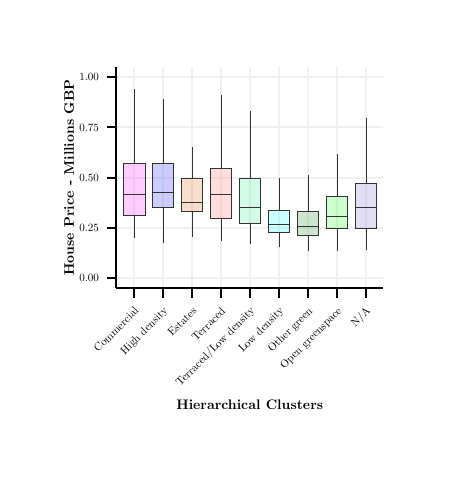
\begin{tikzpicture}[x=1pt,y=1pt]
\definecolor{fillColor}{RGB}{255,255,255}
\path[use as bounding box,fill=fillColor,fill opacity=0.00] (0,0) rectangle (142.64,152.15);
\begin{scope}
\path[clip] (  0.00,  0.00) rectangle (142.64,152.15);
\definecolor{fillColor}{RGB}{255,255,255}

\path[fill=fillColor] (  0.00,  0.00) rectangle (142.64,152.15);
\end{scope}
\begin{scope}
\path[clip] ( 32.06, 58.04) rectangle (128.41,137.92);
\definecolor{fillColor}{RGB}{255,255,255}

\path[fill=fillColor] ( 32.06, 58.04) rectangle (128.41,137.92);
\definecolor{drawColor}{gray}{0.94}

\path[draw=drawColor,line width= 0.7pt,line join=round] ( 32.06, 61.67) --
	(128.41, 61.67);

\path[draw=drawColor,line width= 0.7pt,line join=round] ( 32.06, 79.82) --
	(128.41, 79.82);

\path[draw=drawColor,line width= 0.7pt,line join=round] ( 32.06, 97.98) --
	(128.41, 97.98);

\path[draw=drawColor,line width= 0.7pt,line join=round] ( 32.06,116.13) --
	(128.41,116.13);

\path[draw=drawColor,line width= 0.7pt,line join=round] ( 32.06,134.29) --
	(128.41,134.29);

\path[draw=drawColor,line width= 0.7pt,line join=round] ( 38.34, 58.04) --
	( 38.34,137.92);

\path[draw=drawColor,line width= 0.7pt,line join=round] ( 48.82, 58.04) --
	( 48.82,137.92);

\path[draw=drawColor,line width= 0.7pt,line join=round] ( 59.29, 58.04) --
	( 59.29,137.92);

\path[draw=drawColor,line width= 0.7pt,line join=round] ( 69.76, 58.04) --
	( 69.76,137.92);

\path[draw=drawColor,line width= 0.7pt,line join=round] ( 80.23, 58.04) --
	( 80.23,137.92);

\path[draw=drawColor,line width= 0.7pt,line join=round] ( 90.71, 58.04) --
	( 90.71,137.92);

\path[draw=drawColor,line width= 0.7pt,line join=round] (101.18, 58.04) --
	(101.18,137.92);

\path[draw=drawColor,line width= 0.7pt,line join=round] (111.65, 58.04) --
	(111.65,137.92);

\path[draw=drawColor,line width= 0.7pt,line join=round] (122.13, 58.04) --
	(122.13,137.92);
\definecolor{drawColor}{gray}{0.20}

\path[draw=drawColor,line width= 0.1pt,line join=round] ( 48.82,103.24) -- ( 48.82,126.44);

\path[draw=drawColor,line width= 0.1pt,line join=round] ( 48.82, 87.14) -- ( 48.82, 74.44);
\definecolor{fillColor}{RGB}{0,0,255}

\path[draw=drawColor,line width= 0.1pt,fill=fillColor,fill opacity=0.20] ( 44.89,103.24) --
	( 44.89, 87.14) --
	( 52.74, 87.14) --
	( 52.74,103.24) --
	( 44.89,103.24) --
	cycle;

\path[draw=drawColor,line width= 0.1pt] ( 44.89, 92.86) -- ( 52.74, 92.86);

\path[draw=drawColor,line width= 0.1pt,line join=round] ( 38.34,103.32) -- ( 38.34,129.97);

\path[draw=drawColor,line width= 0.1pt,line join=round] ( 38.34, 84.55) -- ( 38.34, 76.26);
\definecolor{fillColor}{RGB}{255,0,255}

\path[draw=drawColor,line width= 0.1pt,fill=fillColor,fill opacity=0.20] ( 34.41,103.32) --
	( 34.41, 84.55) --
	( 42.27, 84.55) --
	( 42.27,103.32) --
	( 34.41,103.32) --
	cycle;

\path[draw=drawColor,line width= 0.1pt] ( 34.41, 91.86) -- ( 42.27, 91.86);

\path[draw=drawColor,line width= 0.1pt,line join=round] ( 90.71, 86.06) -- ( 90.71, 97.67);

\path[draw=drawColor,line width= 0.1pt,line join=round] ( 90.71, 78.30) -- ( 90.71, 73.01);
\definecolor{fillColor}{RGB}{0,255,255}

\path[draw=drawColor,line width= 0.1pt,fill=fillColor,fill opacity=0.20] ( 86.78, 86.06) --
	( 86.78, 78.30) --
	( 94.64, 78.30) --
	( 94.64, 86.06) --
	( 86.78, 86.06) --
	cycle;

\path[draw=drawColor,line width= 0.1pt] ( 86.78, 81.18) -- ( 94.64, 81.18);

\path[draw=drawColor,line width= 0.1pt,line join=round] (101.18, 85.91) -- (101.18, 98.90);

\path[draw=drawColor,line width= 0.1pt,line join=round] (101.18, 77.02) -- (101.18, 71.47);
\definecolor{fillColor}{RGB}{0,128,0}

\path[draw=drawColor,line width= 0.1pt,fill=fillColor,fill opacity=0.20] ( 97.25, 85.91) --
	( 97.25, 77.02) --
	(105.11, 77.02) --
	(105.11, 85.91) --
	( 97.25, 85.91) --
	cycle;

\path[draw=drawColor,line width= 0.1pt] ( 97.25, 80.33) -- (105.11, 80.33);

\path[draw=drawColor,line width= 0.1pt,line join=round] ( 69.76,101.48) -- ( 69.76,127.67);

\path[draw=drawColor,line width= 0.1pt,line join=round] ( 69.76, 83.26) -- ( 69.76, 75.16);
\definecolor{fillColor}{RGB}{255,85,85}

\path[draw=drawColor,line width= 0.1pt,fill=fillColor,fill opacity=0.20] ( 65.83,101.48) --
	( 65.83, 83.26) --
	( 73.69, 83.26) --
	( 73.69,101.48) --
	( 65.83,101.48) --
	cycle;

\path[draw=drawColor,line width= 0.1pt] ( 65.83, 91.97) -- ( 73.69, 91.97);

\path[draw=drawColor,line width= 0.1pt,line join=round] ( 80.23, 97.82) -- ( 80.23,122.18);

\path[draw=drawColor,line width= 0.1pt,line join=round] ( 80.23, 81.35) -- ( 80.23, 73.80);
\definecolor{fillColor}{RGB}{37,229,137}

\path[draw=drawColor,line width= 0.1pt,fill=fillColor,fill opacity=0.20] ( 76.31, 97.82) --
	( 76.31, 81.35) --
	( 84.16, 81.35) --
	( 84.16, 97.82) --
	( 76.31, 97.82) --
	cycle;

\path[draw=drawColor,line width= 0.1pt] ( 76.31, 87.25) -- ( 84.16, 87.25);

\path[draw=drawColor,line width= 0.1pt,line join=round] (111.65, 91.31) -- (111.65,106.49);

\path[draw=drawColor,line width= 0.1pt,line join=round] (111.65, 79.62) -- (111.65, 71.36);
\definecolor{fillColor}{RGB}{0,255,0}

\path[draw=drawColor,line width= 0.1pt,fill=fillColor,fill opacity=0.20] (107.73, 91.31) --
	(107.73, 79.62) --
	(115.58, 79.62) --
	(115.58, 91.31) --
	(107.73, 91.31) --
	cycle;

\path[draw=drawColor,line width= 0.1pt] (107.73, 84.20) -- (115.58, 84.20);

\path[draw=drawColor,line width= 0.1pt,line join=round] ( 59.29, 97.69) -- ( 59.29,108.95);

\path[draw=drawColor,line width= 0.1pt,line join=round] ( 59.29, 85.82) -- ( 59.29, 76.38);
\definecolor{fillColor}{RGB}{212,85,0}

\path[draw=drawColor,line width= 0.1pt,fill=fillColor,fill opacity=0.20] ( 55.36, 97.69) --
	( 55.36, 85.82) --
	( 63.22, 85.82) --
	( 63.22, 97.69) --
	( 55.36, 97.69) --
	cycle;

\path[draw=drawColor,line width= 0.1pt] ( 55.36, 89.21) -- ( 63.22, 89.21);

\path[draw=drawColor,line width= 0.1pt,line join=round] (122.13, 95.82) -- (122.13,119.64);

\path[draw=drawColor,line width= 0.1pt,line join=round] (122.13, 79.83) -- (122.13, 71.79);
\definecolor{fillColor}{RGB}{106,90,205}

\path[draw=drawColor,line width= 0.1pt,fill=fillColor,fill opacity=0.20] (118.20, 95.82) --
	(118.20, 79.83) --
	(126.06, 79.83) --
	(126.06, 95.82) --
	(118.20, 95.82) --
	cycle;

\path[draw=drawColor,line width= 0.1pt] (118.20, 87.22) -- (126.06, 87.22);

\path[] ( 32.06, 58.04) rectangle (128.41,137.92);
\end{scope}
\begin{scope}
\path[clip] (  0.00,  0.00) rectangle (142.64,152.15);
\definecolor{drawColor}{RGB}{0,0,0}

\path[draw=drawColor,line width= 0.7pt,line join=round] ( 32.06, 58.04) --
	( 32.06,137.92);
\end{scope}
\begin{scope}
\path[clip] (  0.00,  0.00) rectangle (142.64,152.15);
\definecolor{drawColor}{RGB}{0,0,0}

\node[text=drawColor,anchor=base east,inner sep=0pt, outer sep=0pt, scale=  0.40] at ( 25.76, 60.29) {0.00};

\node[text=drawColor,anchor=base east,inner sep=0pt, outer sep=0pt, scale=  0.40] at ( 25.76, 78.45) {0.25};

\node[text=drawColor,anchor=base east,inner sep=0pt, outer sep=0pt, scale=  0.40] at ( 25.76, 96.60) {0.50};

\node[text=drawColor,anchor=base east,inner sep=0pt, outer sep=0pt, scale=  0.40] at ( 25.76,114.76) {0.75};

\node[text=drawColor,anchor=base east,inner sep=0pt, outer sep=0pt, scale=  0.40] at ( 25.76,132.91) {1.00};
\end{scope}
\begin{scope}
\path[clip] (  0.00,  0.00) rectangle (142.64,152.15);
\definecolor{drawColor}{RGB}{0,0,0}

\path[draw=drawColor,line width= 0.7pt,line join=round] ( 28.56, 61.67) --
	( 32.06, 61.67);

\path[draw=drawColor,line width= 0.7pt,line join=round] ( 28.56, 79.82) --
	( 32.06, 79.82);

\path[draw=drawColor,line width= 0.7pt,line join=round] ( 28.56, 97.98) --
	( 32.06, 97.98);

\path[draw=drawColor,line width= 0.7pt,line join=round] ( 28.56,116.13) --
	( 32.06,116.13);

\path[draw=drawColor,line width= 0.7pt,line join=round] ( 28.56,134.29) --
	( 32.06,134.29);
\end{scope}
\begin{scope}
\path[clip] (  0.00,  0.00) rectangle (142.64,152.15);
\definecolor{drawColor}{RGB}{0,0,0}

\path[draw=drawColor,line width= 0.7pt,line join=round] ( 32.06, 58.04) --
	(128.41, 58.04);
\end{scope}
\begin{scope}
\path[clip] (  0.00,  0.00) rectangle (142.64,152.15);
\definecolor{drawColor}{RGB}{0,0,0}

\path[draw=drawColor,line width= 0.7pt,line join=round] ( 38.34, 54.54) --
	( 38.34, 58.04);

\path[draw=drawColor,line width= 0.7pt,line join=round] ( 48.82, 54.54) --
	( 48.82, 58.04);

\path[draw=drawColor,line width= 0.7pt,line join=round] ( 59.29, 54.54) --
	( 59.29, 58.04);

\path[draw=drawColor,line width= 0.7pt,line join=round] ( 69.76, 54.54) --
	( 69.76, 58.04);

\path[draw=drawColor,line width= 0.7pt,line join=round] ( 80.23, 54.54) --
	( 80.23, 58.04);

\path[draw=drawColor,line width= 0.7pt,line join=round] ( 90.71, 54.54) --
	( 90.71, 58.04);

\path[draw=drawColor,line width= 0.7pt,line join=round] (101.18, 54.54) --
	(101.18, 58.04);

\path[draw=drawColor,line width= 0.7pt,line join=round] (111.65, 54.54) --
	(111.65, 58.04);

\path[draw=drawColor,line width= 0.7pt,line join=round] (122.13, 54.54) --
	(122.13, 58.04);
\end{scope}
\begin{scope}
\path[clip] (  0.00,  0.00) rectangle (142.64,152.15);
\definecolor{drawColor}{RGB}{0,0,0}

\node[text=drawColor,rotate= 45.00,anchor=base east,inner sep=0pt, outer sep=0pt, scale=  0.40] at ( 40.27, 49.51) {Commercial};

\node[text=drawColor,rotate= 45.00,anchor=base east,inner sep=0pt, outer sep=0pt, scale=  0.40] at ( 50.74, 49.51) {High density};

\node[text=drawColor,rotate= 45.00,anchor=base east,inner sep=0pt, outer sep=0pt, scale=  0.40] at ( 61.22, 49.51) {Estates};

\node[text=drawColor,rotate= 45.00,anchor=base east,inner sep=0pt, outer sep=0pt, scale=  0.40] at ( 71.69, 49.51) {Terraced};

\node[text=drawColor,rotate= 45.00,anchor=base east,inner sep=0pt, outer sep=0pt, scale=  0.40] at ( 82.16, 49.51) {Terraced/Low density};

\node[text=drawColor,rotate= 45.00,anchor=base east,inner sep=0pt, outer sep=0pt, scale=  0.40] at ( 92.64, 49.51) {Low density};

\node[text=drawColor,rotate= 45.00,anchor=base east,inner sep=0pt, outer sep=0pt, scale=  0.40] at (103.11, 49.51) {Other green};

\node[text=drawColor,rotate= 45.00,anchor=base east,inner sep=0pt, outer sep=0pt, scale=  0.40] at (113.58, 49.51) {Open greenspace};

\node[text=drawColor,rotate= 45.00,anchor=base east,inner sep=0pt, outer sep=0pt, scale=  0.40] at (124.06, 49.51) {N/A};
\end{scope}
\begin{scope}
\path[clip] (  0.00,  0.00) rectangle (142.64,152.15);
\definecolor{drawColor}{RGB}{0,0,0}

\node[text=drawColor,anchor=base,inner sep=0pt, outer sep=0pt, scale=  0.50] at ( 80.23, 14.03) {\bfseries Hierarchical Clusters};
\end{scope}
\begin{scope}
\path[clip] (  0.00,  0.00) rectangle (142.64,152.15);
\definecolor{drawColor}{RGB}{0,0,0}

\node[text=drawColor,rotate= 90.00,anchor=base,inner sep=0pt, outer sep=0pt, scale=  0.50] at ( 16.70, 97.98) {\bfseries House Price - Millions GBP};
\end{scope}
\end{tikzpicture}
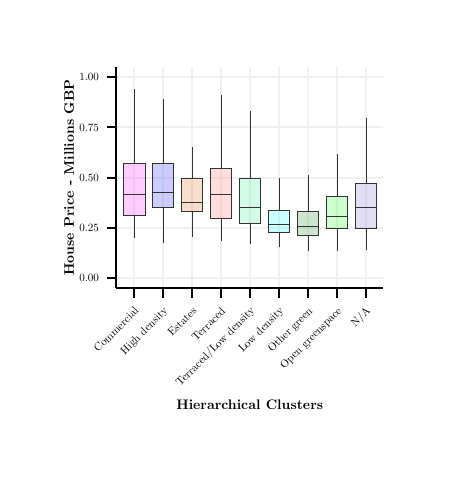
\begin{tikzpicture}[x=1pt,y=1pt]
\definecolor{fillColor}{RGB}{255,255,255}
\path[use as bounding box,fill=fillColor,fill opacity=0.00] (0,0) rectangle (142.64,152.15);
\begin{scope}
\path[clip] (  0.00,  0.00) rectangle (142.64,152.15);
\definecolor{fillColor}{RGB}{255,255,255}

\path[fill=fillColor] (  0.00,  0.00) rectangle (142.64,152.15);
\end{scope}
\begin{scope}
\path[clip] ( 32.06, 58.04) rectangle (128.41,137.92);
\definecolor{fillColor}{RGB}{255,255,255}

\path[fill=fillColor] ( 32.06, 58.04) rectangle (128.41,137.92);
\definecolor{drawColor}{gray}{0.94}

\path[draw=drawColor,line width= 0.7pt,line join=round] ( 32.06, 61.67) --
	(128.41, 61.67);

\path[draw=drawColor,line width= 0.7pt,line join=round] ( 32.06, 79.82) --
	(128.41, 79.82);

\path[draw=drawColor,line width= 0.7pt,line join=round] ( 32.06, 97.98) --
	(128.41, 97.98);

\path[draw=drawColor,line width= 0.7pt,line join=round] ( 32.06,116.13) --
	(128.41,116.13);

\path[draw=drawColor,line width= 0.7pt,line join=round] ( 32.06,134.29) --
	(128.41,134.29);

\path[draw=drawColor,line width= 0.7pt,line join=round] ( 38.34, 58.04) --
	( 38.34,137.92);

\path[draw=drawColor,line width= 0.7pt,line join=round] ( 48.82, 58.04) --
	( 48.82,137.92);

\path[draw=drawColor,line width= 0.7pt,line join=round] ( 59.29, 58.04) --
	( 59.29,137.92);

\path[draw=drawColor,line width= 0.7pt,line join=round] ( 69.76, 58.04) --
	( 69.76,137.92);

\path[draw=drawColor,line width= 0.7pt,line join=round] ( 80.23, 58.04) --
	( 80.23,137.92);

\path[draw=drawColor,line width= 0.7pt,line join=round] ( 90.71, 58.04) --
	( 90.71,137.92);

\path[draw=drawColor,line width= 0.7pt,line join=round] (101.18, 58.04) --
	(101.18,137.92);

\path[draw=drawColor,line width= 0.7pt,line join=round] (111.65, 58.04) --
	(111.65,137.92);

\path[draw=drawColor,line width= 0.7pt,line join=round] (122.13, 58.04) --
	(122.13,137.92);
\definecolor{drawColor}{gray}{0.20}

\path[draw=drawColor,line width= 0.1pt,line join=round] ( 48.82,103.24) -- ( 48.82,126.44);

\path[draw=drawColor,line width= 0.1pt,line join=round] ( 48.82, 87.14) -- ( 48.82, 74.44);
\definecolor{fillColor}{RGB}{0,0,255}

\path[draw=drawColor,line width= 0.1pt,fill=fillColor,fill opacity=0.20] ( 44.89,103.24) --
	( 44.89, 87.14) --
	( 52.74, 87.14) --
	( 52.74,103.24) --
	( 44.89,103.24) --
	cycle;

\path[draw=drawColor,line width= 0.1pt] ( 44.89, 92.86) -- ( 52.74, 92.86);

\path[draw=drawColor,line width= 0.1pt,line join=round] ( 38.34,103.32) -- ( 38.34,129.97);

\path[draw=drawColor,line width= 0.1pt,line join=round] ( 38.34, 84.55) -- ( 38.34, 76.26);
\definecolor{fillColor}{RGB}{255,0,255}

\path[draw=drawColor,line width= 0.1pt,fill=fillColor,fill opacity=0.20] ( 34.41,103.32) --
	( 34.41, 84.55) --
	( 42.27, 84.55) --
	( 42.27,103.32) --
	( 34.41,103.32) --
	cycle;

\path[draw=drawColor,line width= 0.1pt] ( 34.41, 91.86) -- ( 42.27, 91.86);

\path[draw=drawColor,line width= 0.1pt,line join=round] ( 90.71, 86.06) -- ( 90.71, 97.67);

\path[draw=drawColor,line width= 0.1pt,line join=round] ( 90.71, 78.30) -- ( 90.71, 73.01);
\definecolor{fillColor}{RGB}{0,255,255}

\path[draw=drawColor,line width= 0.1pt,fill=fillColor,fill opacity=0.20] ( 86.78, 86.06) --
	( 86.78, 78.30) --
	( 94.64, 78.30) --
	( 94.64, 86.06) --
	( 86.78, 86.06) --
	cycle;

\path[draw=drawColor,line width= 0.1pt] ( 86.78, 81.18) -- ( 94.64, 81.18);

\path[draw=drawColor,line width= 0.1pt,line join=round] (101.18, 85.91) -- (101.18, 98.90);

\path[draw=drawColor,line width= 0.1pt,line join=round] (101.18, 77.02) -- (101.18, 71.47);
\definecolor{fillColor}{RGB}{0,128,0}

\path[draw=drawColor,line width= 0.1pt,fill=fillColor,fill opacity=0.20] ( 97.25, 85.91) --
	( 97.25, 77.02) --
	(105.11, 77.02) --
	(105.11, 85.91) --
	( 97.25, 85.91) --
	cycle;

\path[draw=drawColor,line width= 0.1pt] ( 97.25, 80.33) -- (105.11, 80.33);

\path[draw=drawColor,line width= 0.1pt,line join=round] ( 69.76,101.48) -- ( 69.76,127.67);

\path[draw=drawColor,line width= 0.1pt,line join=round] ( 69.76, 83.26) -- ( 69.76, 75.16);
\definecolor{fillColor}{RGB}{255,85,85}

\path[draw=drawColor,line width= 0.1pt,fill=fillColor,fill opacity=0.20] ( 65.83,101.48) --
	( 65.83, 83.26) --
	( 73.69, 83.26) --
	( 73.69,101.48) --
	( 65.83,101.48) --
	cycle;

\path[draw=drawColor,line width= 0.1pt] ( 65.83, 91.97) -- ( 73.69, 91.97);

\path[draw=drawColor,line width= 0.1pt,line join=round] ( 80.23, 97.82) -- ( 80.23,122.18);

\path[draw=drawColor,line width= 0.1pt,line join=round] ( 80.23, 81.35) -- ( 80.23, 73.80);
\definecolor{fillColor}{RGB}{37,229,137}

\path[draw=drawColor,line width= 0.1pt,fill=fillColor,fill opacity=0.20] ( 76.31, 97.82) --
	( 76.31, 81.35) --
	( 84.16, 81.35) --
	( 84.16, 97.82) --
	( 76.31, 97.82) --
	cycle;

\path[draw=drawColor,line width= 0.1pt] ( 76.31, 87.25) -- ( 84.16, 87.25);

\path[draw=drawColor,line width= 0.1pt,line join=round] (111.65, 91.31) -- (111.65,106.49);

\path[draw=drawColor,line width= 0.1pt,line join=round] (111.65, 79.62) -- (111.65, 71.36);
\definecolor{fillColor}{RGB}{0,255,0}

\path[draw=drawColor,line width= 0.1pt,fill=fillColor,fill opacity=0.20] (107.73, 91.31) --
	(107.73, 79.62) --
	(115.58, 79.62) --
	(115.58, 91.31) --
	(107.73, 91.31) --
	cycle;

\path[draw=drawColor,line width= 0.1pt] (107.73, 84.20) -- (115.58, 84.20);

\path[draw=drawColor,line width= 0.1pt,line join=round] ( 59.29, 97.69) -- ( 59.29,108.95);

\path[draw=drawColor,line width= 0.1pt,line join=round] ( 59.29, 85.82) -- ( 59.29, 76.38);
\definecolor{fillColor}{RGB}{212,85,0}

\path[draw=drawColor,line width= 0.1pt,fill=fillColor,fill opacity=0.20] ( 55.36, 97.69) --
	( 55.36, 85.82) --
	( 63.22, 85.82) --
	( 63.22, 97.69) --
	( 55.36, 97.69) --
	cycle;

\path[draw=drawColor,line width= 0.1pt] ( 55.36, 89.21) -- ( 63.22, 89.21);

\path[draw=drawColor,line width= 0.1pt,line join=round] (122.13, 95.82) -- (122.13,119.64);

\path[draw=drawColor,line width= 0.1pt,line join=round] (122.13, 79.83) -- (122.13, 71.79);
\definecolor{fillColor}{RGB}{106,90,205}

\path[draw=drawColor,line width= 0.1pt,fill=fillColor,fill opacity=0.20] (118.20, 95.82) --
	(118.20, 79.83) --
	(126.06, 79.83) --
	(126.06, 95.82) --
	(118.20, 95.82) --
	cycle;

\path[draw=drawColor,line width= 0.1pt] (118.20, 87.22) -- (126.06, 87.22);

\path[] ( 32.06, 58.04) rectangle (128.41,137.92);
\end{scope}
\begin{scope}
\path[clip] (  0.00,  0.00) rectangle (142.64,152.15);
\definecolor{drawColor}{RGB}{0,0,0}

\path[draw=drawColor,line width= 0.7pt,line join=round] ( 32.06, 58.04) --
	( 32.06,137.92);
\end{scope}
\begin{scope}
\path[clip] (  0.00,  0.00) rectangle (142.64,152.15);
\definecolor{drawColor}{RGB}{0,0,0}

\node[text=drawColor,anchor=base east,inner sep=0pt, outer sep=0pt, scale=  0.40] at ( 25.76, 60.29) {0.00};

\node[text=drawColor,anchor=base east,inner sep=0pt, outer sep=0pt, scale=  0.40] at ( 25.76, 78.45) {0.25};

\node[text=drawColor,anchor=base east,inner sep=0pt, outer sep=0pt, scale=  0.40] at ( 25.76, 96.60) {0.50};

\node[text=drawColor,anchor=base east,inner sep=0pt, outer sep=0pt, scale=  0.40] at ( 25.76,114.76) {0.75};

\node[text=drawColor,anchor=base east,inner sep=0pt, outer sep=0pt, scale=  0.40] at ( 25.76,132.91) {1.00};
\end{scope}
\begin{scope}
\path[clip] (  0.00,  0.00) rectangle (142.64,152.15);
\definecolor{drawColor}{RGB}{0,0,0}

\path[draw=drawColor,line width= 0.7pt,line join=round] ( 28.56, 61.67) --
	( 32.06, 61.67);

\path[draw=drawColor,line width= 0.7pt,line join=round] ( 28.56, 79.82) --
	( 32.06, 79.82);

\path[draw=drawColor,line width= 0.7pt,line join=round] ( 28.56, 97.98) --
	( 32.06, 97.98);

\path[draw=drawColor,line width= 0.7pt,line join=round] ( 28.56,116.13) --
	( 32.06,116.13);

\path[draw=drawColor,line width= 0.7pt,line join=round] ( 28.56,134.29) --
	( 32.06,134.29);
\end{scope}
\begin{scope}
\path[clip] (  0.00,  0.00) rectangle (142.64,152.15);
\definecolor{drawColor}{RGB}{0,0,0}

\path[draw=drawColor,line width= 0.7pt,line join=round] ( 32.06, 58.04) --
	(128.41, 58.04);
\end{scope}
\begin{scope}
\path[clip] (  0.00,  0.00) rectangle (142.64,152.15);
\definecolor{drawColor}{RGB}{0,0,0}

\path[draw=drawColor,line width= 0.7pt,line join=round] ( 38.34, 54.54) --
	( 38.34, 58.04);

\path[draw=drawColor,line width= 0.7pt,line join=round] ( 48.82, 54.54) --
	( 48.82, 58.04);

\path[draw=drawColor,line width= 0.7pt,line join=round] ( 59.29, 54.54) --
	( 59.29, 58.04);

\path[draw=drawColor,line width= 0.7pt,line join=round] ( 69.76, 54.54) --
	( 69.76, 58.04);

\path[draw=drawColor,line width= 0.7pt,line join=round] ( 80.23, 54.54) --
	( 80.23, 58.04);

\path[draw=drawColor,line width= 0.7pt,line join=round] ( 90.71, 54.54) --
	( 90.71, 58.04);

\path[draw=drawColor,line width= 0.7pt,line join=round] (101.18, 54.54) --
	(101.18, 58.04);

\path[draw=drawColor,line width= 0.7pt,line join=round] (111.65, 54.54) --
	(111.65, 58.04);

\path[draw=drawColor,line width= 0.7pt,line join=round] (122.13, 54.54) --
	(122.13, 58.04);
\end{scope}
\begin{scope}
\path[clip] (  0.00,  0.00) rectangle (142.64,152.15);
\definecolor{drawColor}{RGB}{0,0,0}

\node[text=drawColor,rotate= 45.00,anchor=base east,inner sep=0pt, outer sep=0pt, scale=  0.40] at ( 40.27, 49.51) {Commercial};

\node[text=drawColor,rotate= 45.00,anchor=base east,inner sep=0pt, outer sep=0pt, scale=  0.40] at ( 50.74, 49.51) {High density};

\node[text=drawColor,rotate= 45.00,anchor=base east,inner sep=0pt, outer sep=0pt, scale=  0.40] at ( 61.22, 49.51) {Estates};

\node[text=drawColor,rotate= 45.00,anchor=base east,inner sep=0pt, outer sep=0pt, scale=  0.40] at ( 71.69, 49.51) {Terraced};

\node[text=drawColor,rotate= 45.00,anchor=base east,inner sep=0pt, outer sep=0pt, scale=  0.40] at ( 82.16, 49.51) {Terraced/Low density};

\node[text=drawColor,rotate= 45.00,anchor=base east,inner sep=0pt, outer sep=0pt, scale=  0.40] at ( 92.64, 49.51) {Low density};

\node[text=drawColor,rotate= 45.00,anchor=base east,inner sep=0pt, outer sep=0pt, scale=  0.40] at (103.11, 49.51) {Other green};

\node[text=drawColor,rotate= 45.00,anchor=base east,inner sep=0pt, outer sep=0pt, scale=  0.40] at (113.58, 49.51) {Open greenspace};

\node[text=drawColor,rotate= 45.00,anchor=base east,inner sep=0pt, outer sep=0pt, scale=  0.40] at (124.06, 49.51) {N/A};
\end{scope}
\begin{scope}
\path[clip] (  0.00,  0.00) rectangle (142.64,152.15);
\definecolor{drawColor}{RGB}{0,0,0}

\node[text=drawColor,anchor=base,inner sep=0pt, outer sep=0pt, scale=  0.50] at ( 80.23, 14.03) {\bfseries Hierarchical Clusters};
\end{scope}
\begin{scope}
\path[clip] (  0.00,  0.00) rectangle (142.64,152.15);
\definecolor{drawColor}{RGB}{0,0,0}

\node[text=drawColor,rotate= 90.00,anchor=base,inner sep=0pt, outer sep=0pt, scale=  0.50] at ( 16.70, 97.98) {\bfseries House Price - Millions GBP};
\end{scope}
\end{tikzpicture}
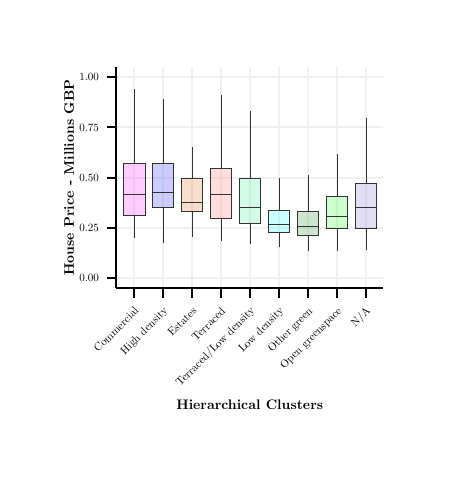
\begin{tikzpicture}[x=1pt,y=1pt]
\definecolor{fillColor}{RGB}{255,255,255}
\path[use as bounding box,fill=fillColor,fill opacity=0.00] (0,0) rectangle (142.64,152.15);
\begin{scope}
\path[clip] (  0.00,  0.00) rectangle (142.64,152.15);
\definecolor{fillColor}{RGB}{255,255,255}

\path[fill=fillColor] (  0.00,  0.00) rectangle (142.64,152.15);
\end{scope}
\begin{scope}
\path[clip] ( 32.06, 58.04) rectangle (128.41,137.92);
\definecolor{fillColor}{RGB}{255,255,255}

\path[fill=fillColor] ( 32.06, 58.04) rectangle (128.41,137.92);
\definecolor{drawColor}{gray}{0.94}

\path[draw=drawColor,line width= 0.7pt,line join=round] ( 32.06, 61.67) --
	(128.41, 61.67);

\path[draw=drawColor,line width= 0.7pt,line join=round] ( 32.06, 79.82) --
	(128.41, 79.82);

\path[draw=drawColor,line width= 0.7pt,line join=round] ( 32.06, 97.98) --
	(128.41, 97.98);

\path[draw=drawColor,line width= 0.7pt,line join=round] ( 32.06,116.13) --
	(128.41,116.13);

\path[draw=drawColor,line width= 0.7pt,line join=round] ( 32.06,134.29) --
	(128.41,134.29);

\path[draw=drawColor,line width= 0.7pt,line join=round] ( 38.34, 58.04) --
	( 38.34,137.92);

\path[draw=drawColor,line width= 0.7pt,line join=round] ( 48.82, 58.04) --
	( 48.82,137.92);

\path[draw=drawColor,line width= 0.7pt,line join=round] ( 59.29, 58.04) --
	( 59.29,137.92);

\path[draw=drawColor,line width= 0.7pt,line join=round] ( 69.76, 58.04) --
	( 69.76,137.92);

\path[draw=drawColor,line width= 0.7pt,line join=round] ( 80.23, 58.04) --
	( 80.23,137.92);

\path[draw=drawColor,line width= 0.7pt,line join=round] ( 90.71, 58.04) --
	( 90.71,137.92);

\path[draw=drawColor,line width= 0.7pt,line join=round] (101.18, 58.04) --
	(101.18,137.92);

\path[draw=drawColor,line width= 0.7pt,line join=round] (111.65, 58.04) --
	(111.65,137.92);

\path[draw=drawColor,line width= 0.7pt,line join=round] (122.13, 58.04) --
	(122.13,137.92);
\definecolor{drawColor}{gray}{0.20}

\path[draw=drawColor,line width= 0.1pt,line join=round] ( 48.82,103.24) -- ( 48.82,126.44);

\path[draw=drawColor,line width= 0.1pt,line join=round] ( 48.82, 87.14) -- ( 48.82, 74.44);
\definecolor{fillColor}{RGB}{0,0,255}

\path[draw=drawColor,line width= 0.1pt,fill=fillColor,fill opacity=0.20] ( 44.89,103.24) --
	( 44.89, 87.14) --
	( 52.74, 87.14) --
	( 52.74,103.24) --
	( 44.89,103.24) --
	cycle;

\path[draw=drawColor,line width= 0.1pt] ( 44.89, 92.86) -- ( 52.74, 92.86);

\path[draw=drawColor,line width= 0.1pt,line join=round] ( 38.34,103.32) -- ( 38.34,129.97);

\path[draw=drawColor,line width= 0.1pt,line join=round] ( 38.34, 84.55) -- ( 38.34, 76.26);
\definecolor{fillColor}{RGB}{255,0,255}

\path[draw=drawColor,line width= 0.1pt,fill=fillColor,fill opacity=0.20] ( 34.41,103.32) --
	( 34.41, 84.55) --
	( 42.27, 84.55) --
	( 42.27,103.32) --
	( 34.41,103.32) --
	cycle;

\path[draw=drawColor,line width= 0.1pt] ( 34.41, 91.86) -- ( 42.27, 91.86);

\path[draw=drawColor,line width= 0.1pt,line join=round] ( 90.71, 86.06) -- ( 90.71, 97.67);

\path[draw=drawColor,line width= 0.1pt,line join=round] ( 90.71, 78.30) -- ( 90.71, 73.01);
\definecolor{fillColor}{RGB}{0,255,255}

\path[draw=drawColor,line width= 0.1pt,fill=fillColor,fill opacity=0.20] ( 86.78, 86.06) --
	( 86.78, 78.30) --
	( 94.64, 78.30) --
	( 94.64, 86.06) --
	( 86.78, 86.06) --
	cycle;

\path[draw=drawColor,line width= 0.1pt] ( 86.78, 81.18) -- ( 94.64, 81.18);

\path[draw=drawColor,line width= 0.1pt,line join=round] (101.18, 85.91) -- (101.18, 98.90);

\path[draw=drawColor,line width= 0.1pt,line join=round] (101.18, 77.02) -- (101.18, 71.47);
\definecolor{fillColor}{RGB}{0,128,0}

\path[draw=drawColor,line width= 0.1pt,fill=fillColor,fill opacity=0.20] ( 97.25, 85.91) --
	( 97.25, 77.02) --
	(105.11, 77.02) --
	(105.11, 85.91) --
	( 97.25, 85.91) --
	cycle;

\path[draw=drawColor,line width= 0.1pt] ( 97.25, 80.33) -- (105.11, 80.33);

\path[draw=drawColor,line width= 0.1pt,line join=round] ( 69.76,101.48) -- ( 69.76,127.67);

\path[draw=drawColor,line width= 0.1pt,line join=round] ( 69.76, 83.26) -- ( 69.76, 75.16);
\definecolor{fillColor}{RGB}{255,85,85}

\path[draw=drawColor,line width= 0.1pt,fill=fillColor,fill opacity=0.20] ( 65.83,101.48) --
	( 65.83, 83.26) --
	( 73.69, 83.26) --
	( 73.69,101.48) --
	( 65.83,101.48) --
	cycle;

\path[draw=drawColor,line width= 0.1pt] ( 65.83, 91.97) -- ( 73.69, 91.97);

\path[draw=drawColor,line width= 0.1pt,line join=round] ( 80.23, 97.82) -- ( 80.23,122.18);

\path[draw=drawColor,line width= 0.1pt,line join=round] ( 80.23, 81.35) -- ( 80.23, 73.80);
\definecolor{fillColor}{RGB}{37,229,137}

\path[draw=drawColor,line width= 0.1pt,fill=fillColor,fill opacity=0.20] ( 76.31, 97.82) --
	( 76.31, 81.35) --
	( 84.16, 81.35) --
	( 84.16, 97.82) --
	( 76.31, 97.82) --
	cycle;

\path[draw=drawColor,line width= 0.1pt] ( 76.31, 87.25) -- ( 84.16, 87.25);

\path[draw=drawColor,line width= 0.1pt,line join=round] (111.65, 91.31) -- (111.65,106.49);

\path[draw=drawColor,line width= 0.1pt,line join=round] (111.65, 79.62) -- (111.65, 71.36);
\definecolor{fillColor}{RGB}{0,255,0}

\path[draw=drawColor,line width= 0.1pt,fill=fillColor,fill opacity=0.20] (107.73, 91.31) --
	(107.73, 79.62) --
	(115.58, 79.62) --
	(115.58, 91.31) --
	(107.73, 91.31) --
	cycle;

\path[draw=drawColor,line width= 0.1pt] (107.73, 84.20) -- (115.58, 84.20);

\path[draw=drawColor,line width= 0.1pt,line join=round] ( 59.29, 97.69) -- ( 59.29,108.95);

\path[draw=drawColor,line width= 0.1pt,line join=round] ( 59.29, 85.82) -- ( 59.29, 76.38);
\definecolor{fillColor}{RGB}{212,85,0}

\path[draw=drawColor,line width= 0.1pt,fill=fillColor,fill opacity=0.20] ( 55.36, 97.69) --
	( 55.36, 85.82) --
	( 63.22, 85.82) --
	( 63.22, 97.69) --
	( 55.36, 97.69) --
	cycle;

\path[draw=drawColor,line width= 0.1pt] ( 55.36, 89.21) -- ( 63.22, 89.21);

\path[draw=drawColor,line width= 0.1pt,line join=round] (122.13, 95.82) -- (122.13,119.64);

\path[draw=drawColor,line width= 0.1pt,line join=round] (122.13, 79.83) -- (122.13, 71.79);
\definecolor{fillColor}{RGB}{106,90,205}

\path[draw=drawColor,line width= 0.1pt,fill=fillColor,fill opacity=0.20] (118.20, 95.82) --
	(118.20, 79.83) --
	(126.06, 79.83) --
	(126.06, 95.82) --
	(118.20, 95.82) --
	cycle;

\path[draw=drawColor,line width= 0.1pt] (118.20, 87.22) -- (126.06, 87.22);

\path[] ( 32.06, 58.04) rectangle (128.41,137.92);
\end{scope}
\begin{scope}
\path[clip] (  0.00,  0.00) rectangle (142.64,152.15);
\definecolor{drawColor}{RGB}{0,0,0}

\path[draw=drawColor,line width= 0.7pt,line join=round] ( 32.06, 58.04) --
	( 32.06,137.92);
\end{scope}
\begin{scope}
\path[clip] (  0.00,  0.00) rectangle (142.64,152.15);
\definecolor{drawColor}{RGB}{0,0,0}

\node[text=drawColor,anchor=base east,inner sep=0pt, outer sep=0pt, scale=  0.40] at ( 25.76, 60.29) {0.00};

\node[text=drawColor,anchor=base east,inner sep=0pt, outer sep=0pt, scale=  0.40] at ( 25.76, 78.45) {0.25};

\node[text=drawColor,anchor=base east,inner sep=0pt, outer sep=0pt, scale=  0.40] at ( 25.76, 96.60) {0.50};

\node[text=drawColor,anchor=base east,inner sep=0pt, outer sep=0pt, scale=  0.40] at ( 25.76,114.76) {0.75};

\node[text=drawColor,anchor=base east,inner sep=0pt, outer sep=0pt, scale=  0.40] at ( 25.76,132.91) {1.00};
\end{scope}
\begin{scope}
\path[clip] (  0.00,  0.00) rectangle (142.64,152.15);
\definecolor{drawColor}{RGB}{0,0,0}

\path[draw=drawColor,line width= 0.7pt,line join=round] ( 28.56, 61.67) --
	( 32.06, 61.67);

\path[draw=drawColor,line width= 0.7pt,line join=round] ( 28.56, 79.82) --
	( 32.06, 79.82);

\path[draw=drawColor,line width= 0.7pt,line join=round] ( 28.56, 97.98) --
	( 32.06, 97.98);

\path[draw=drawColor,line width= 0.7pt,line join=round] ( 28.56,116.13) --
	( 32.06,116.13);

\path[draw=drawColor,line width= 0.7pt,line join=round] ( 28.56,134.29) --
	( 32.06,134.29);
\end{scope}
\begin{scope}
\path[clip] (  0.00,  0.00) rectangle (142.64,152.15);
\definecolor{drawColor}{RGB}{0,0,0}

\path[draw=drawColor,line width= 0.7pt,line join=round] ( 32.06, 58.04) --
	(128.41, 58.04);
\end{scope}
\begin{scope}
\path[clip] (  0.00,  0.00) rectangle (142.64,152.15);
\definecolor{drawColor}{RGB}{0,0,0}

\path[draw=drawColor,line width= 0.7pt,line join=round] ( 38.34, 54.54) --
	( 38.34, 58.04);

\path[draw=drawColor,line width= 0.7pt,line join=round] ( 48.82, 54.54) --
	( 48.82, 58.04);

\path[draw=drawColor,line width= 0.7pt,line join=round] ( 59.29, 54.54) --
	( 59.29, 58.04);

\path[draw=drawColor,line width= 0.7pt,line join=round] ( 69.76, 54.54) --
	( 69.76, 58.04);

\path[draw=drawColor,line width= 0.7pt,line join=round] ( 80.23, 54.54) --
	( 80.23, 58.04);

\path[draw=drawColor,line width= 0.7pt,line join=round] ( 90.71, 54.54) --
	( 90.71, 58.04);

\path[draw=drawColor,line width= 0.7pt,line join=round] (101.18, 54.54) --
	(101.18, 58.04);

\path[draw=drawColor,line width= 0.7pt,line join=round] (111.65, 54.54) --
	(111.65, 58.04);

\path[draw=drawColor,line width= 0.7pt,line join=round] (122.13, 54.54) --
	(122.13, 58.04);
\end{scope}
\begin{scope}
\path[clip] (  0.00,  0.00) rectangle (142.64,152.15);
\definecolor{drawColor}{RGB}{0,0,0}

\node[text=drawColor,rotate= 45.00,anchor=base east,inner sep=0pt, outer sep=0pt, scale=  0.40] at ( 40.27, 49.51) {Commercial};

\node[text=drawColor,rotate= 45.00,anchor=base east,inner sep=0pt, outer sep=0pt, scale=  0.40] at ( 50.74, 49.51) {High density};

\node[text=drawColor,rotate= 45.00,anchor=base east,inner sep=0pt, outer sep=0pt, scale=  0.40] at ( 61.22, 49.51) {Estates};

\node[text=drawColor,rotate= 45.00,anchor=base east,inner sep=0pt, outer sep=0pt, scale=  0.40] at ( 71.69, 49.51) {Terraced};

\node[text=drawColor,rotate= 45.00,anchor=base east,inner sep=0pt, outer sep=0pt, scale=  0.40] at ( 82.16, 49.51) {Terraced/Low density};

\node[text=drawColor,rotate= 45.00,anchor=base east,inner sep=0pt, outer sep=0pt, scale=  0.40] at ( 92.64, 49.51) {Low density};

\node[text=drawColor,rotate= 45.00,anchor=base east,inner sep=0pt, outer sep=0pt, scale=  0.40] at (103.11, 49.51) {Other green};

\node[text=drawColor,rotate= 45.00,anchor=base east,inner sep=0pt, outer sep=0pt, scale=  0.40] at (113.58, 49.51) {Open greenspace};

\node[text=drawColor,rotate= 45.00,anchor=base east,inner sep=0pt, outer sep=0pt, scale=  0.40] at (124.06, 49.51) {N/A};
\end{scope}
\begin{scope}
\path[clip] (  0.00,  0.00) rectangle (142.64,152.15);
\definecolor{drawColor}{RGB}{0,0,0}

\node[text=drawColor,anchor=base,inner sep=0pt, outer sep=0pt, scale=  0.50] at ( 80.23, 14.03) {\bfseries Hierarchical Clusters};
\end{scope}
\begin{scope}
\path[clip] (  0.00,  0.00) rectangle (142.64,152.15);
\definecolor{drawColor}{RGB}{0,0,0}

\node[text=drawColor,rotate= 90.00,anchor=base,inner sep=0pt, outer sep=0pt, scale=  0.50] at ( 16.70, 97.98) {\bfseries House Price - Millions GBP};
\end{scope}
\end{tikzpicture}
